\documentclass[12pt,a4paper]{article}
%\documentclass[8pt]{beamer}
%\usetheme{default}
%\usepackage[font=small,format=plain,labelfont=bf,up,textfont=it,up]{caption}
\usepackage{setspace}
\usepackage{graphicx}
\usepackage{epstopdf}
%\usepackage{natbib}
%\usepackage[num,overcite]{abntex2cite}

%\usepackage{hyperref}
\usepackage[hidelinks]{hyperref}
\usepackage[alf]{abntex2cite}
%\citebrackets[]

%\bibpunct{(}{)}{;}{a}{}{,}
\usepackage[brazil]{babel}
\usepackage[utf8]{inputenc}
\usepackage {enumerate}
\usepackage{latexsym}
\usepackage{amsmath}
\usepackage{amsthm}
%\usepackage[T1]{fontenc}
%\usepackage{fetamont}
%\usepackage[num]{abntcite}
\usepackage{ mathrsfs }
\usepackage{subfigure}

%\setcitestyle{aysep={,}} 

\newcommand{\farcm}{\mbox{\ensuremath{.\mkern-4mu^\prime}}}%
\newcommand{\farcs}{\mbox{\ensuremath{.\!\!^{\prime\prime}}}}
\newcommand{\ii }{\'{\i}}
\newcommand{\cc }{\c c}
\newcommand{\cca}{\c ca }
\newcommand{\ao}{\~ao }
\newcommand{\cao}{\c c\~ao }
\newcommand{\oes}{\~oes }
\newcommand{\coes}{\c c\~oes }
\newcommand{\eq}{\begin{equation}}
\newcommand{\feq}{\end{equation}}
\newcommand{\dm}{\begin{displaymath}}
\newcommand{\fdm}{\end{displaymath}}
\newcommand{\eqn}{\begin{eqnarray}}
\newcommand{\feqn}{\end{eqnarray}}
\newcommand{\grau}{^{\circ}}
\newcommand{\ba}{\arrowvert_{t_1}^{t_2}}
\newcommand{\bc}{\arrowvert_{0^{\circ} {\rm C}}^{t_2}}
\newcommand{\bb}{\arrowvert_{0^{\circ} {\rm C}}^{t_1}}
\newcommand{\Ms}{$\mathrm{M}_{\odot}$}
%\renewcommand{\labelitemiv}{$-$}
\usepackage{amssymb}
\newcommand{\reg}[1]{#1$^{\tiny{\circledR}}$}
%\usepackage[hmargin=2cm,vmargin=2.5cm,bmargin=2cm]{geometry}
\usepackage[top=3cm, bottom=2cm, left=3cm, right=2cm,asymmetric]{geometry} 
\renewcommand{\baselinestretch}{1.5}

\usepackage{times}

\usepackage{float}

%Arial
%\usepackage{helvet}
%\renewcommand{\familydefault}{\sfdefault}

%Times New Roman
%\usepackage{mathptmx}

%\topmargin -1.5cm
%\leftmargin -2cm
%\rightmargin -2cm
%\oddsidemargin -0.7cm
%\textwidth 16cm
%\textheight 24cm
%\hoffset -1cm 

\usepackage{chngcntr}
%\counterwithout{figure}{chapter}

%\usepackage{fancyhdr}
%
%\fancypagestyle{mypagestyle}{
%\fancyhf{}
%\renewcommand{\headrulewidth}{0.5pt}
%
%\fancyhead[EL]{\normalsize \textsl{\nouppercase{\rightmark}}}
%\fancyhead[OL]{\normalsize \textsl{\nouppercase{\leftmark}}}
%\fancyhead[OR,ER]{}
%\cfoot{\thepage}
%}
%
%%\pagestyle{mypagestyle}

\usepackage[portuguese, boxed, ruled]{algorithm2e}
\usepackage{algorithmic}

\newtheorem{theorem}{Teorema}[section]
\newtheorem{definition}{Definição}[section]
%\newtheorem{lemma}{Lema}[chapter]
%\newtheorem{remark}{Observação}[chapter]

\renewcommand{\qedsymbol}{$\blacksquare$}

\usepackage{epic}
\usepackage{arydshln}
\providecommand{\sin}{} \renewcommand{\sin}{\hspace{2pt}\mathrm{sen}}
\numberwithin{equation}{section}
\usepackage{chngcntr}
%\counterwithout{equation}{section} % undo numbering system provided by phstyle.cls
%\counterwithin{equation}{chapter}
\counterwithin{table}{section}

\usepackage{multirow}
\usepackage{booktabs}

\setcounter{secnumdepth}{3}

\usepackage{tikz}
\usetikzlibrary{fit, shapes, arrows}
\usetikzlibrary{arrows.meta}
\usetikzlibrary{calc,patterns,angles,quotes}
\newcommand{\tikzMarkAngle}[3]{                                                
\tikzAngleOfLine#1#2{\AngleStart}                                              
\tikzAngleOfLine#1#3{\AngleEnd}                                                
\draw #1+(\AngleStart:0.15cm) arc (\AngleStart:\AngleEnd:0.15cm);              
}                                                                              


\tikzstyle{block} = [draw, fill=white, rectangle, 
    minimum height=3em, minimum width=6em, text width=2cm,align = center]
\tikzstyle{sum} = [draw, fill=white, circle, node distance=1cm]
\tikzstyle{input} = [coordinate]
\tikzstyle{output} = [coordinate]
\tikzstyle{pinstyle} = [pin edge={to-,thin,black}]

\tikzstyle{block1} = [draw, fill=white, rectangle, 
    minimum height=3em, minimum width=1em, text width=1cm,align = center]
\tikzstyle{sum} = [draw, fill=white, circle, node distance=1cm]
\tikzstyle{input} = [coordinate]
\tikzstyle{output} = [coordinate]
\tikzstyle{pinstyle} = [pin edge={to-,thin,black}]

\begin{document}
\pagenumbering{Roman}
% CAPA

\thispagestyle{empty}
\hspace{-1cm}
\begin{minipage}{0.35\textwidth}
%\begin{flushleft}
\vspace{-2cm}
  \begin{figure}[H]
    
\includegraphics[scale=0.07]{figures/UFMG-logo.png}
  \end{figure}
%\end{flushleft}  
\end{minipage}
\begin{minipage}{0.7\textwidth}
\textbf{UNIVERSIDADE FEDERAL DE MINAS GERAIS} \\
\textbf{PROGRAMA DE PÓS-GRADUAÇÃO EM ENGENHARIA ELÉTRICA}\\
\end{minipage}


\vspace{30mm}
\begin{center}
\textbf{
LUIZ ALBERTO QUEIROZ CORDOVIL JÚNIOR \\
RODRIGO FARIAS ARAÚJO}
\end{center}

\vspace{50 mm}
\begin{center}
\textbf{SISTEMAS NEBULOSOS: EXERCÍCIO COMPUTACIONAL 2}\\
\end{center}

\vspace{85mm}

\begin{center}
\textbf{Belo Horizonte - MG, 2017}
\end{center}
\thispagestyle{empty}
\newpage

%CONTRA-CAPA

\thispagestyle{empty}

\vspace{3 mm}
\begin{center}
\textbf{
LUIZ ALBERTO QUEIROZ CORDOVIL JÚNIOR \\
RODRIGO FARIAS ARAÚJO}
\end{center}

\vspace{25 mm}
\begin{center}
\textbf{EFFECT OF RULE WEIGHTS IN FUZYY RULE-BASED CLASSIFICATION SYSTEMS}\\
\end{center}

\vspace{30 mm}

\vspace{35mm}
\hspace{8cm}\begin{minipage}[r]{0.45\linewidth}
Relatório apresentado como requisito parcial para obtenção de aprovação na disciplina Sistemas Nebulosos do Programa de Pós-Graduação em Engenharia Elétrica, na Universidade Federal de Minas Gerais.\\ 
\\
Prof. Dr. André Paim Lemos
\end{minipage}

\vspace{50mm}
\begin{center}
\textbf{Belo Horizonte - MG, 2017}
\end{center}

\thispagestyle{empty}
\newpage
\tableofcontents
\newpage
\listoffigures
%\newpage
%\listoftables
\newpage
\pagenumbering{arabic}

%\documentclass[12pt,a4paper]{article}
%%\documentclass[8pt]{beamer}
%%\usetheme{default}
%%\usepackage[font=small,format=plain,labelfont=bf,up,textfont=it,up]{caption}
%%\usepackage{setspace}
%\usepackage{graphicx}
%\usepackage{epstopdf}
%\usepackage{natbib}
%\bibpunct{(}{)}{;}{a}{}{,}
%\usepackage[brazil]{babel}
%\usepackage[utf8]{inputenc}
%\usepackage {enumerate}
%\usepackage{latexsym}
%\usepackage{amsmath}
%%\usepackage[T1]{fontenc}
%%\usepackage{fetamont}
%%\usepackage[num]{abntcite}
%\usepackage{ mathrsfs }
%\usepackage{subfigure}
%\usepackage{helvet}
%\renewcommand{\familydefault}{\sfdefault}
%
%\newcommand{\farcm}{\mbox{\ensuremath{.\mkern-4mu^\prime}}}%
%\newcommand{\farcs}{\mbox{\ensuremath{.\!\!^{\prime\prime}}}}
%\newcommand{\ii }{\'{\i}}
%\newcommand{\cc }{\c c}
%\newcommand{\cca}{\c ca }
%\newcommand{\ao}{\~ao }
%\newcommand{\cao}{\c c\~ao }
%\newcommand{\oes}{\~oes }
%\newcommand{\coes}{\c c\~oes }
%\newcommand{\eq}{\begin{equation}}
%\newcommand{\feq}{\end{equation}}
%\newcommand{\dm}{\begin{displaymath}}
%\newcommand{\fdm}{\end{displaymath}}
%\newcommand{\eqn}{\begin{eqnarray}}
%\newcommand{\feqn}{\end{eqnarray}}
%\newcommand{\grau}{^{\circ}}
%\newcommand{\ba}{\arrowvert_{t_1}^{t_2}}
%\newcommand{\bc}{\arrowvert_{0^{\circ} {\rm C}}^{t_2}}
%\newcommand{\bb}{\arrowvert_{0^{\circ} {\rm C}}^{t_1}}
%\newcommand{\Ms}{$\mathrm{M}_{\odot}$}
%%\renewcommand{\labelitemiv}{$-$}
%\usepackage{amssymb}
%\newcommand{\reg}[1]{#1$^{\tiny{\circledR}}$}
%\usepackage[top=3cm, bottom=2cm, left=3cm, right=2cm,asymmetric]{geometry} 
%\renewcommand{\baselinestretch}{1.5}
%%\topmargin -1.5cm
%%\leftmargin -2cm
%%\rightmargin -2cm
%%\oddsidemargin -0.7cm
%%\textwidth 16cm
%%\textheight 24cm
%%\hoffset -1cm 
%
%\usepackage{epic}
%\usepackage{arydshln}
%\providecommand{\sin}{} \renewcommand{\sin}{\hspace{2pt}\mathrm{sen}}
%\numberwithin{equation}{section}

{\abstract
Este trabalho apresenta a reprodução da metodologia e dos procedimentos experimentais realizados no artigo de Ishibuchi, H. e Nakashima, T. [1], denominado \textit{Effect of Rule Weights in Fuzzy Rule-Based Classification Systems}, em que são avaliados os efeitos de ponderação de regras em sistemas de classificação fuzzy. A metodologia considera que os valores linguísticos antecedentes de cada classe tem uma única classe consequente, a partir da observação de grau de compatibilidade e de certeza, quando da classificação de padrões. Os autores concluem que sistemas de classificação fuzzy com alta desempenho podem ser projetados apenas através do uso de ponderação de regras com graus de certeza, o que é equivalente a técnica de modificação de funções de pertinência de valores linguísticos antecedentes.}
\newpage

\section{Introdução}

De maneira geral os problemas de classificação são aproximações baseadas em dados  no sentido de mapear classes de um conjunto de variáveis. Em sistemas baseados em regras fuzzy, a identificação de padrões e consequente classificação destes a partir de um número finito (\textit{n}) de atributos é definido como:

\begin{equation} \label{eq:eq1}
Regra~R_{j}:~Se~x_{1}~ \text{é }A_{j1}~e~...~e~x_{n}~\text{é }A_{jn}~\text{então}~Classe~C_{j},~j=1,2,...,N
\end{equation}
onde:
\begin{itemize}
\item $x={x_{1},...,x_{n}}$: $n-$dimensional vetor de padrões;
\item $A_{ij}$: valor linguístico antecedente, $~(i=1,2,...,n)$;
\item $C_{j}$: classe consequente;
\item $N$: número de regras fuzzy SE-ENTÃO.
\end{itemize}

Na abordagem do artigo a ponderação das regras SE-ENTÃO com os graus de certeza é dada por:
\begin{equation} \label{eq:eq2}
Regra~R_{j}:~Se~x_{i}~\text{é } A_{j1}~e...e~x_{n}~\text{é}~A_{jn}~\text{então}~Classe~C_{j}~\text{com}~CF_{j}, j=1,2,...,N
\end{equation}
onde $CF_{j}$ é o grau de certeza do consequente, $C_{j}$, de cada regra fuzzy SE-ENTÃO $R_{j}$, é um número real no intervalo [0,1].

Para esta aplicação foi utilizada a base de dados \textit{Iris} (1936), do biólogo e estatístico britânico Ronald Fisher, para três espécies da flor \textit{Iris} (\textit{setosa, virginica, versicolor}), com $50$ amostras de cada espécie totalizando $150$ amostras no conjunto de dados. Considera-se o conjunto de dados separáveis pela discriminação das seguintes características:

\begin{itemize}
\item comprimento e largura da sépala;
\item comprimento e largura da pétala.
\end{itemize}

A Figura \ref{fig:data}, ilustra uma representação bi-dimensional da base dados \textit{Iris} considerando apenas duas variáveis dos mesmos, $x_1$ e $x_2$, as quais representam comprimento e largura da sépala, respectivamente.

\begin{figure}[ht]
\centering
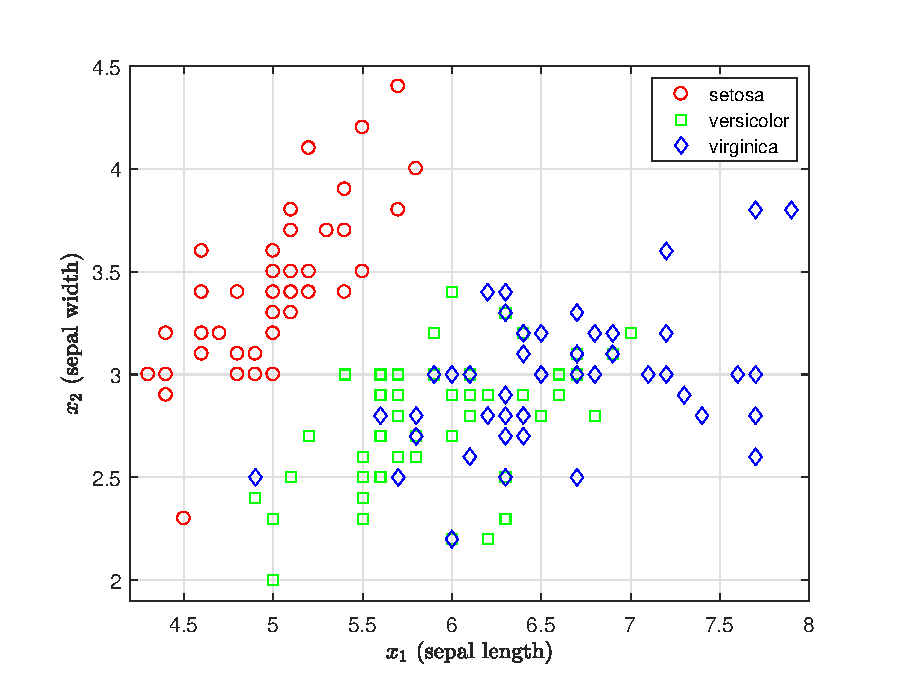
\includegraphics[width=0.7\textwidth]{figures/data.eps}
\caption{Representação bi-dimensional dos dados considerando as variáveis $x_1$ e $x_2$, comprimento e largura da sépala, respectivamente.}
\label{fig:data}
\end{figure}

\section{Metodologia}

O método implementado consiste de uma abordagem de seleção de apenas uma classe, ou classe vencedora, durante a fase de classificação, além de, quando na observação da área de decisão haver fronteiras de classificação tendo em vista as regras fuzzy. Ao ponderar-se estas pelo grau de certeza $C_{j}$:

\begin{equation} \label{eq:eq3}
\sum_{p\in Class~C_{j}} \mu_{j}(x_p)=\max(\sum_{p\in Class~k}\mu(x_{p}):k=1,2,...,c)
\end{equation}
onde: $x_{p}$: número de padrões e $c$: número de classes.

Como pode ser visto na Eq. \eqref{eq:eq3} a classe consequente $C_{j}$ é especificada como a classe dominante no espaço fuzzy correspondente ao antecedente de cada regra fuzzy SE-ENTÃO. Aplicando-se a definição demonstrada na Eq. \eqref{eq:eq2}, um novo padrão $x{p}=(x_{p1},...,x_{pn})$, pode ser classificado a partir de:

\begin{equation} \label{eq:eq4}
\mu_{j}^{ *}(x_{p}).CF_{j}=\max\lbrace\mu_{j}(x_{p}).CF_{j}:~j=1,2,...,N\rbrace
\end{equation}

A classe consequente pode ser determinada a partir de padrões de treinamento, assim como se esta é a classe dominante em determinado subespaço do espaço fuzzy. Como toda regra tem sua própria área de decisão, cujo tamanho é determinado pelo grau de certeza e pelo antecedente linguístico das funções de pertinência, a abordagem realiza mudança na dimensão da área de decisão por ponderação. Neste sentido o grau de certeza pode ser obtido a partir da Eq. \eqref{eq:eq5}.

\begin{equation} \label{eq:eq5}
CF_{j}=\frac{\beta_{Classe~C_{j}}(R_{j})-\overline{\beta}}{\sum_{k=1}^{c}\beta_{Classe~k}(R_{j})}
\end{equation}
onde $C_{j}$ é a classe consequente e:

\begin{equation} \label{eq:eq6}
\overline{\beta}=\frac{\sum_{k\neq C_{j}}\beta_{Classe~k}(R_{j})}{(c-1)}
\end{equation}

As formulações indicadas nas equações \eqref{eq:eq5} e \eqref{eq:eq6} estendem a determinação do grau de certeza para um problema de classificação com $c$ classes.

%\subsection{Procedimentos Computacionais}
\section{Resultados}

Inicialmente o modelo foi descrito através de apenas duas variáveis do conjunto de dados, as quais correspondem ao comprimento e largura da sépala de todas as classes, afim de se visualizar as delimitações das regiões de classificação.

Em seguida, todas as quatro variáveis do conjunto de dados são utilizadas para criação de um modelo de classificação geral. A abordagem empregada consiste na técnica de validação cruzada, onde são utilizados de maneira aleatória $70\%$ dos dados para treinamento e os $30\%$ dos dados restantes para validação do modelo.

Além disso, o número de funções de pertinência para descrição das variáveis linguísticas é alterado de $2$ até $15$ funções de pertinências. Todo o processo é repetido $25$ vezes para um número fixo de funções de pertinência, afim de se obter o erro médio de classificação, desconsiderando a natureza estocástica da escolha dos dados de treinamento de validação.

A escolha do tipo de função de pertinência é a mesma apresenta em [1], funções triangulares igualmente espaçadas. A Figura \ref{fig:membership} ilustra $6$ funções de pertinência para cada uma das variáveis da base de dados \textit{Iris}, considerando as variáveis já normalizadas.

\begin{figure}[ht!]
\centering
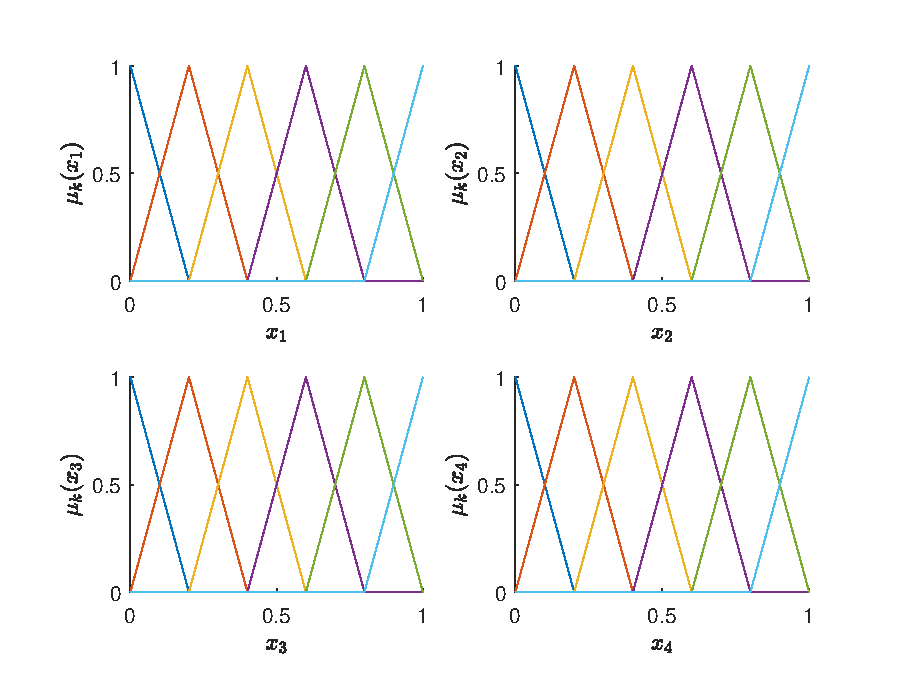
\includegraphics[width=0.9\textwidth]{figures/membership.eps}
\caption{Funções de pertinência para variável do banco de dados \textit{Iris}.}
\label{fig:membership}
\end{figure}

\subsection{Regiões de Classificação}

Como os dados possuem quatro variáveis de entradas, a visualização das regiões de classificação é prejudicada, para exemplificar, apenas duas variáveis, comprimento e largura da sépala, foram utilizadas no treinamento afim de se obter regiões de classificação bi-dimensionais, conforme dito anteriormente.

Nesta etapa, a partir da definição do grau de certeza na observação das características do conjunto de dados, o sistema de classificação converge para uma discriminação das classes (espécies), como uma área de decisão, a partir da especificação de cada regra e da fronteira de classificação.

As Figuras \ref{fig:product} e \ref{fig:minimum} ilustram as regiões de classificação obtidas a partir da utilização das \textit{t-normas}, produto e mínimo, respectivamente. Em ambas as Figuras foram utilizadas $8$ (oito) funções de pertinência triangulares para definição dos antecedentes das variáveis, $x_1$ e $x_2$. O motivo dessa escolha será abordado na Subseção \ref{subsection:training}.

%Conforme indicado na Seção \ref{PC}, como função de duas variáveis, a área de decisão, com a utilização de t-norma, produto, é indicada na Figura \ref{fig:product}:

\begin{figure}[ht!]
\centering
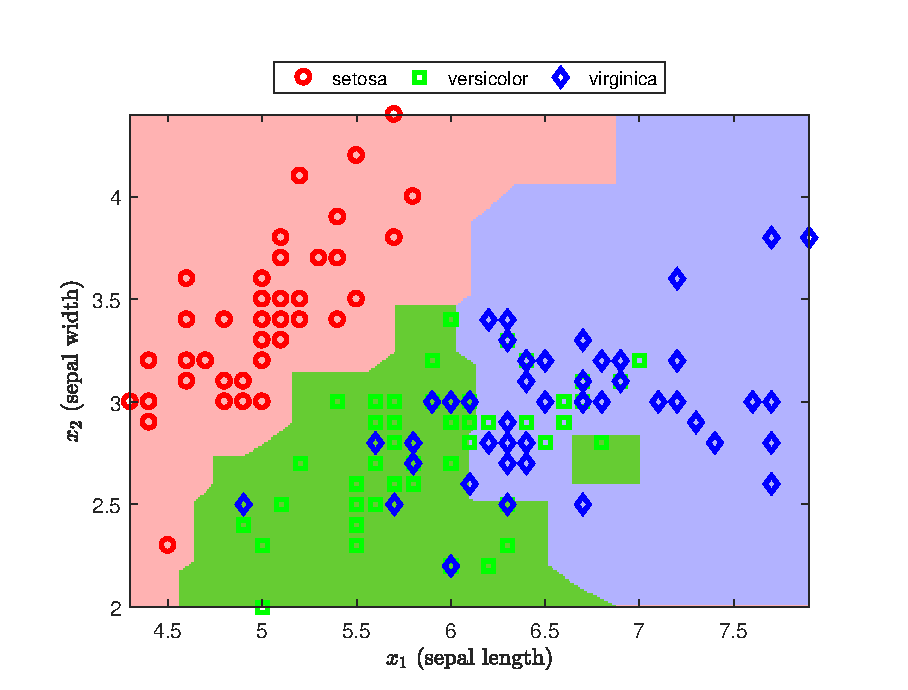
\includegraphics[width=0.7\textwidth]{figures/product.eps}
\caption{Região de classificação usando a t-norma produto.}
\label{fig:product}
\end{figure}

%A região de decisão com a utilização da t-norma, mínimo, é ilustrada na Figura \ref{fig:minimum}:

\begin{figure}[ht!]
\centering
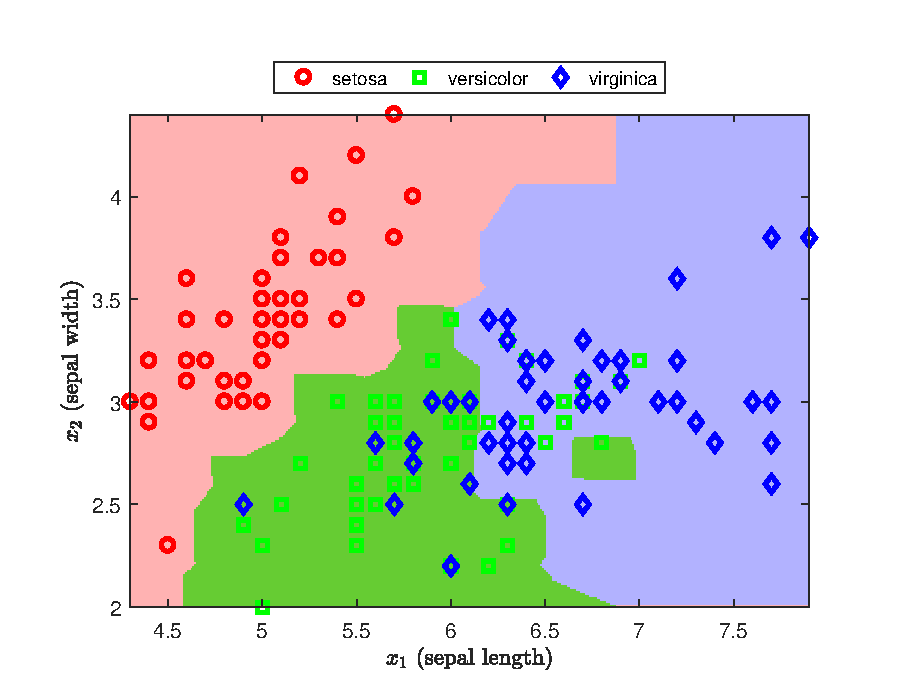
\includegraphics[width=0.7\textwidth]{figures/minimum.eps}
\caption{Região de classificação usando a t-norma mínimo.}
\label{fig:minimum}
\end{figure}

O particionamento do espaço de entrada (variáveis) fornece o suporte para formulação de regras que estejam relacionadas a este subespaço. Em termos práticos, a utilização destes dois tipos de conjunções lógicas, implica na análise das regras, sejam elas condicionais (relação interna entre antecedentes e consequentes) e incondicionais, de maneira geral afirmativas. 

Nota-se que o processo de inferência, ou seja, o processo de avaliação das regras para cada subconjunto fuzzy acaba por estabelecer relações. Neste caso, no sistema de classificação, ao combinar-se o conjunto de dados de entrada, ao menos uma regra deve ser ativada, ponderada pelo grau de certeza.

Além disso, os operadores mínimo e produto algébrico, utilizados como \textit{t-norma} no que se refere a inferência composicional de regras, estabelecem a interseção entre regras para a dedução de uma consequência lógica.

\subsection{Treinamento e Validação}
\label{subsection:training}

Na abordagem computacional, por meio da técnica de validação cruzada, cada conjunto de espécies foi separado de forma aleatória em subconjuntos de treinamento e validação representados, com dimensão de $70\%$ e $30\%$, respectivamente de cada classe de padrões.

Para todas as classes, no total, quatro dados de entrada aplicados a três espécies, com $50$ amostras. Como ferramenta de aprendizagem, os conjuntos de treinamento e validação, foram determinados observando-se os percentuais em $35$ e $15$ amostras, respectivamente, para cada classe $C_{j}$.

Neste sentido, na etapa de treinamento, a partir de aprendizado supervisionado, houve a classificação inicial das amostras, como função da quantidade de regras e dos graus de certeza, no sentido de se estabelecer as condições e parâmetros iniciais do sistema de classificação.

A partir destes, houve a implementação das características de contexto adquiridas na etapa de treinamento, no sentido de aferir-se a performance do sistema de classificação.

Os experimentos foram realizados $25$ vezes, para cada número de funções de pertinência de $2$ até $15$, com o propósito de se observar o limiar de convergência e paridade entre o erro do conjunto de treinamento e erro no conjunto de validação e eliminar a natureza estocástica da escolha do dados de treinamento de validação.

%As amostras foram escolhidas aleatoriamente dentro dos subconjuntos e avaliadas para cada conjunto de regras, por n repetidas vezes.


\begin{figure}[ht]
\centering
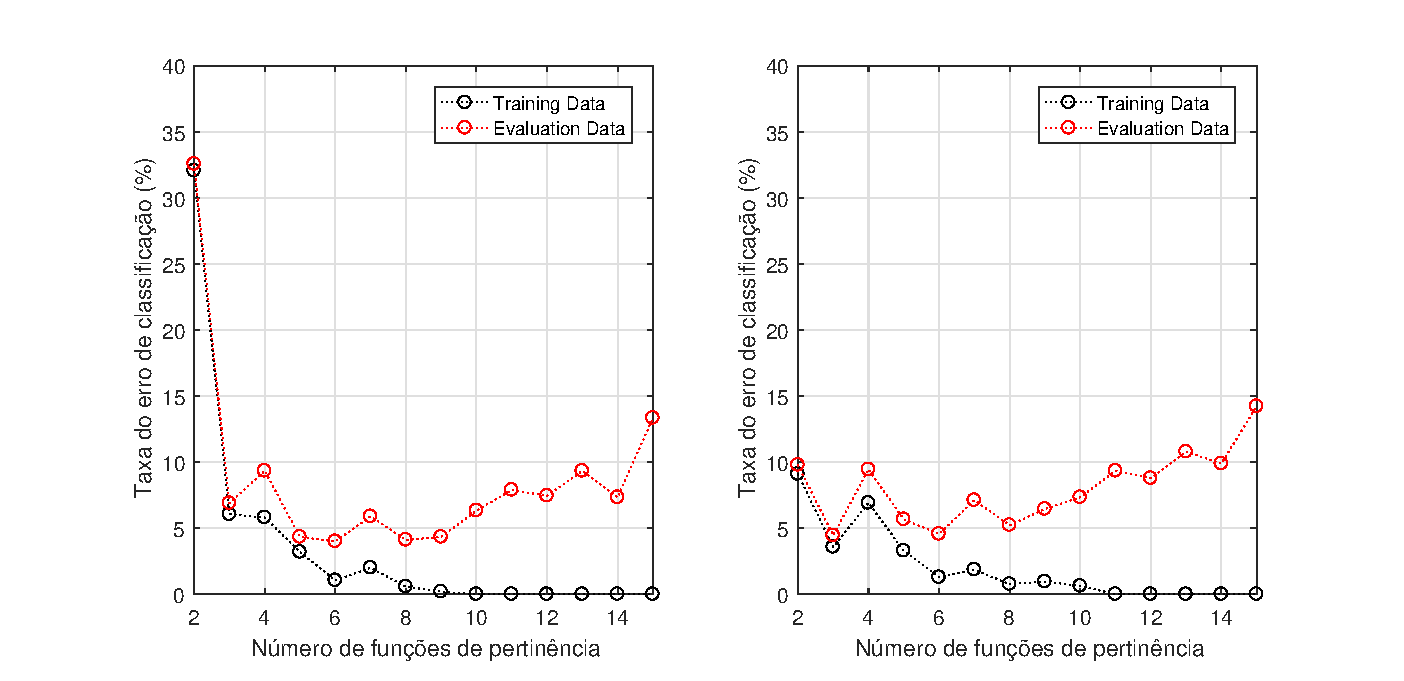
\includegraphics[width=0.7\textwidth]{figures/error.eps}
\caption{Trajetória do erro em relação ao número de funções de pertinência, considerando a avaliação dos dados de treinamento e validação.}
\label{fig:error}
\end{figure}

\newpage
\section{Conclusões}

A utilização de sistemas de classificação baseados em regras ponderadas através de graus de certeza, oferece uma solução baseada em conhecimento dedutivo, o que em termos práticos, implica na sobreposição de uma regra dominante sobre outra no espaço fuzzy, ou seja, na combinação de $n$ regras, pelo menos uma, por inferência composicional, forma a consequência lógica.

Todos os procedimentos realizados no artigo e replicados em simulações compõem base de conhecimento por raciocínio aproximado pelo fato da definição de consequentes a partir de relações de compatibilidade em função dos graus de certeza. Neste sentido as conclusões das conjunções lógicas, seja pelo operador mínimo ou produto como \textit{t-norma}, são baseadas no domínio de uma regra sobre a outra no espaço de decisão, sendo este ponderado pelo grau de certeza.

Assim, o procedimento apresentado em [1], o qual consiste na ponderação de regras SE-ENTÃO a partir de graus de certeza substitui a necessidade de otimização das funções de pertinências empregadas para descrição das variáveis linguísticas.
\newpage

\section*{Referências}
\addcontentsline{toc}{section}{\protect\numberline{}Referências}%

[1] ISHIBUCHI, Hisao; NAKASHIMA, Tomoharu. Effect of rule weights in fuzzy rule-based classification systems. IEEE Transactions on Fuzzy Systems, v. 9, n. 4, p. 506-515, 2001.

\end{document}
